\documentclass[12pt]{exam}		%Doc : https://mirrors.ircam.fr/pub/CTAN/macros/latex/contrib/exam/examdoc.pdf
\printanswers					%Comment this line to hide the answers 
\usepackage[utf8]{inputenc}
\usepackage[T1]{fontenc}
\usepackage[french]{babel}      %Originally for french document, change to english or relevant language

\usepackage{amsmath,amssymb}
\usepackage{multicol}
\usepackage[dvipsnames]{xcolor}
\usepackage[shortlabels]{enumitem}
\usepackage{tikz}
	\usetikzlibrary{fadings}
	\usetikzlibrary{calc}
	
\usepackage{tkz-tab}
\usepackage{pgfplots}

%Format Header and footer
\pagestyle{headandfoot}
\header{\footnotesize Class\\Id number}{\Large\textbf{Name}}
\headrule
\footrule
\setlength{\columnsep}{0.25cm}
%\setlength{\columnseprule}{1pt}
\footer{}{Page \thepage}{}
%\extrafootheight{-2cm}

% Change section command behaviour
\usepackage{titlesec}
\titleformat{\section}[frame]{\Huge\bfseries\filright}{}{2mm}{\centering Chemistry 107 :\ }

% Add a watermark if answers are shown
%\ifprintanswers
%\usepackage{draftwatermark}
%\SetWatermarkColor{red!30}
%\SetWatermarkScale{5}
%\SetWatermarkText{Solution}     %Watermark text
%\fi

%Format the name of each exercise
\qformat{\textbf{Exercice \thequestion~:}\hfill}
\extrawidth{1.5cm}

\begin{document}
\section{Final Exam}

\noindent The 150 pts final exam consists of 14 questions and students have 2 hours to complete the exam.
Answers must be written in the box provided or else no credit is provided. Use the empty
space provided to do your work. A periodic table is provided at the end. Fill in your name along with your
student ID number.
\\

\noindent\textbf{Problem 1: True/False } Determine whether the statement is true or false. (20 pts)
\\
\begin{enumerate}[(a)]
%\item An element is a pure substance that contains only one type of atom. %True
%\item[]\tikz[baseline=1ex]\draw (0,0) rectangle (17cm,5ex);
\item Catalysts speed up the chemical reaction by lowering the activation
  Energy. ($E_A$) %True
\item[]\tikz[baseline=1ex]\draw (0,0) rectangle (17cm,5ex);
%\item Atoms are indivisible and indestructible. %False
%\item[]\tikz[baseline=1ex]\draw (0,0) rectangle (17cm,5ex);
\item The atomic number of a substance is the number of neutrons that an
  element has. %False
\item[]\tikz[baseline=1ex]\draw (0,0) rectangle (17cm,5ex);
\item Photons from red lights have lower energy than violet light. %True
\item[]\tikz[baseline=1ex]\draw (0,0) rectangle (17cm,5ex);
\item As the wavelength of light increases, the photon energy decreases
  as well %True
\item[]\tikz[baseline=1ex]\draw (0,0) rectangle (17cm,5ex);
\item The mass of an atom is the sum of the masses of neutrons, protons, and
  electrons. %True
\item[]\tikz[baseline=1ex]\draw (0,0) rectangle (17cm,5ex);
\item Matter and energy are neither created nor destroyed. %True
\item[]\tikz[baseline=1ex]\draw (0,0) rectangle (17cm,5ex);
%\item All Br{\o}nsted acids are Lewis acids. %True
%\item[]\tikz[baseline=1ex]\draw (0,0) rectangle (17cm,5ex);
%\item Given a solution at concentration $M$, when the volume of the solution
%  is increased by 2 times, then concentration is halved. %True
%\item[]\tikz[baseline=1ex]\draw (0,0) rectangle (17cm,5ex);
%\item Creating metal alloys such as steel and bronze is considered a physical change. %True
%\item[]\tikz[baseline=1ex]\draw (0,0) rectangle (17cm,5ex);
\item Suppose a system is in thermal equilibrium with a heat bath.
  When the temperature of the heat bath increases, the temperature of the
  system increases. %True
\item[]\tikz[baseline=1ex]\draw (0,0) rectangle (17cm,5ex);
\item The boiling point of molecules depends on the strength of
  intermolecular forces. %True
\item[]\tikz[baseline=1ex]\draw (0,0) rectangle (17cm,5ex);
\item Carbon atoms can form more than 4 bonds. %False
\item[]\tikz[baseline=1ex]\draw (0,0) rectangle (17cm,5ex);
\item Boiling of liquids occurs when the vapor pressure of the liquid
  is less than the atmospheric pressure. %False
\item[]\tikz[baseline=1ex]\draw (0,0) rectangle (17cm,5ex);
\end{enumerate}

\newpage

\noindent\textbf{Problem 2: Nomenclature} Provide either the molecular formula or
compound name for the following. (13 pts)
\\
\begin{enumerate}[(a)]
\item Sulfurous acid % H2SO3
\item[]\tikz[baseline=1ex]\draw (0,0) rectangle (17cm,5ex);
\item Chromium(VI) oxide %
\item[]\tikz[baseline=1ex]\draw (0,0) rectangle (17cm,5ex);
\item V$_2$O$_5$ % Vanadium(V) oxide
\item[]\tikz[baseline=1ex]\draw (0,0) rectangle (17cm,5ex);
\item Vanadium(V) acetate %V(C2H3O2)5
\item[]\tikz[baseline=1ex]\draw (0,0) rectangle (17cm,5ex);
\item Sr(C$_2$H$_3$O$_2$) %Strontium Acetate
\item[]\tikz[baseline=1ex]\draw (0,0) rectangle (17cm,5ex);
\item HClO$_3$ %Cloric acid
\item[]\tikz[baseline=1ex]\draw (0,0) rectangle (17cm,5ex);
\item (NH$_4$)$_2$SO$_4$ %Ammonium Sulfate
\item[]\tikz[baseline=1ex]\draw (0,0) rectangle (17cm,5ex);
\item Carbonic acid %H2CO3
\item[]\tikz[baseline=1ex]\draw (0,0) rectangle (17cm,5ex);
\item Sodium bicarbonate %NaHCO3
\item[]\tikz[baseline=1ex]\draw (0,0) rectangle (17cm,5ex);
\item CaO
\item[]\tikz[baseline=1ex]\draw (0,0) rectangle (17cm,5ex);
\item SF$_4$
\item[]\tikz[baseline=1ex]\draw (0,0) rectangle (17cm,5ex);
\item BeCl$_2$
\item[]\tikz[baseline=1ex]\draw (0,0) rectangle (17cm,5ex);
\item Sodium permanganate
\item[]\tikz[baseline=1ex]\draw (0,0) rectangle (17cm,5ex);
\end{enumerate}

\newpage

\noindent\textbf{Problem 3: Molarity} Magnesium sulfate (MgSO$_4$) can
be used as a soaking solution to relieve minor sprains, bruises, muscle aches
or discomfort, joint stiffness or soreness, and tired feet. Answer the
following questions and report all results to 3 significant figures. (12 pts)
\\
\begin{enumerate}[(a)]
\item Determine the mass percent of each element in MgSO$_4$.
  \vspace{2in}
\item[]\tikz[baseline=1ex]\draw (0,0) rectangle (17cm,5ex);
\item A scientist attempts to prepare 5.00L of 2M MgSO$_4$. How many grams of
  MgSO$_4$ is needed?
  \vspace{2in}
\item[]\tikz[baseline=1ex]\draw (0,0) rectangle (17cm,5ex);
\item Suppose the solution in part b) needs to be diluted to make
  2.00L of 0.25M MgSO$_5$, how much volume in L is needed from 2M MgSO$_4$?
  \vspace{2in}
\item[]\tikz[baseline=1ex]\draw (0,0) rectangle (17cm,5ex);
\end{enumerate}

\newpage

\noindent\textbf{Problem 4: Thermal Equilibrium} 700.0g of aluminum (Al)
metal block is heated to 350.0$^\circ$C and then, dropped into
1,000.g of water (H$_2$O) at 0$^\circ$C. The specific heats of H$_2$Oand Alare
4.184 J/(g $^\circ$C) and 0.890 J/(g $^\circ$C), respectively. Determine the
final temperature at which the Al and H$_2$O are in thermal equilibrium. Report to
4 significant figures. (12 pts)

\vspace{2.5in}

\tikz[baseline=1ex]\draw (0,0) rectangle (17cm,5ex);
\\

\noindent\textbf{Problem 5: Relative Atomic Mass} Boron has only two naturally occurring
isotopes (Boron-10 and Boron-11). The mass of Boron-10 is 10.01294 amu and the mass of
Boron-11 is 11.00931 amu. The relative abundances of Boron-10 and Boron-11 are 0.1998
and 0.8002. Report to 3 significant figures. Calculate the relative atomic mass. (4 pts)
\vspace{3.5in}
\\
\tikz[baseline=1ex]\draw (0,0) rectangle (17cm,5ex);

\newpage

\noindent\textbf{Problem 6: Atoms and Ions} Complete the table with the symbol,
atomic number $Z$, atomic mass $A$, number of protons ($p^+$), number of electrons
$e^-$, number of neutrons $n$, and charge. (10 pts)
\\
\begin{table}[hbpt]
  \centering
  \Huge
  \begin{tabular}{c|cccccc}
    Symbol & $Z$ & $A$ & $p^+$ & $e^-$ & $n$ & Charge \\
    \hline\hline
    Sn      & 50 & & 50 &  & 63 & \\
    O$^{2-}$ & & 16 & & & & \\
    & 26 & & & & 31 & 2+ \\
    & 19 & & & 19 & 16 & 1+ \\
    Xe & & 130 & & & \\
    \hline
  \end{tabular}
\end{table}

\noindent\textbf{Problem 7: Empirical and Molecular Formulas} Answer the following questions.
(10 pts)
\\
\begin{enumerate}[(a)]
\item Mining iron requires removing impurities such as sulfur. Suppose a sample
  is found to contain $63.52\%$ iron and $36.48\%$ sulfur. Determine the empirical
  formula  %FeS
  \vspace{1.5in}
\item[]\tikz[baseline=1ex]\draw (0,0) rectangle (17cm,5ex);
\item In class, we dealt with many different hydrocarbons. Determine the molecular
  formula of the compound with an empirical formula of CH and a molar mass of 78.110g/mol.
  %C6H6
  \vspace{1.5in}
\item[]\tikz[baseline=1ex]\draw (0,0) rectangle (17cm,5ex);
\end{enumerate}

\newpage

\noindent\textbf{Problem 8: Drawing Lewis Structures}
Draw the Lewis structures for the following compounds, identify the
geometric shape, and whether the compound is polar or nonpolar. If there
are resonance structures, then include them in your answer.(18 pts)

\begin{enumerate}[(a)]
\item HSCN
\item[]\tikz[baseline=1ex]\draw (0,0) rectangle (17.5cm,34ex);
\item BeCl
\item[]\tikz[baseline=1ex]\draw (0,0) rectangle (17.5cm,34ex);
\item O$_3$
\item[]\tikz[baseline=1ex]\draw (0,0) rectangle (17.5cm,34ex);
\item NH$_3$
\item[]\tikz[baseline=1ex]\draw (0,0) rectangle (17.5cm,35ex);
\item H$_3$O$^+$
\item[]\tikz[baseline=1ex]\draw (0,0) rectangle (17.5cm,35ex);
\item CO$_3^{2-}$
\item[]\tikz[baseline=1ex]\draw (0,0) rectangle (17.5cm,35ex);
\end{enumerate}

\newpage

\noindent\textbf{Problem 9: Applications of Ideal Gas Law} The
following questions are applying the ideal gas law. Report values
to 3 significant figures. (12 pts)

\begin{enumerate}[(a)]
\item Suppose a fixed amount of H$_2$ gas is stored inside a container. Sketch a graph
  describing the relationship between temperature and pressure.
  Describe this relationship.
\item[]\tikz[baseline=1ex]\draw (0,0) rectangle (17.5cm,40ex);
\item What is the density of laughing gas, dinitrogen monoxide, N2O, at a temperature
  of 325K and a pressure of 113.0 kPa?
  \vspace{1.75in}
\item[]\tikz[baseline=1ex]\draw (0,0) rectangle (17.5cm,5ex);
\item A sample of H$_2$ gas occupies 1.50L at 80.0$^\circ$C and 3.00atm. What
  volume does H$_2$ gas will it occupy at 185$^\circ$C and 5.00 atm?
  \vspace{1.75in}
\item[]\tikz[baseline=1ex]\draw (0,0) rectangle (17.5cm,5ex);
\end{enumerate}

\newpage

\noindent\textbf{Problem 10: Ideal Gas and Chemical Equation} Automobile air bags
are inflated with nitrogen gas (N$_2$), which is formed by the decomposition of solid
sodium azide (NaN$_3$). The other product is sodium metal (Na). (6 pts)

\begin{enumerate}[(a)]
\item Write the balanced chemical equation of the decomposition of sodium azide
  including states.
\item[]\tikz[baseline=1ex]\draw (0,0) rectangle (17.5cm,5ex);
\item Calculate the volume of nitrogen gas at 27 °C and 756 torr formed by the
  decomposition of 125 g of sodium azide.
  \vspace{2.5in}
\item[]\tikz[baseline=1ex]\draw (0,0) rectangle (17.5cm,5ex);
\end{enumerate}

\noindent\textbf{Problem 11: Acid-Base Reaction} To neutralize sulfuric acid
(H$_2$SO$_4$), sodium hydroxide (NaOH) is used to form a salt and water. Report to
3 significant figures. (6 pts)
\\
\begin{enumerate}[(a)]
\item Write the balanced chemical equation including states.
\item[]\tikz[baseline=1ex]\draw (0,0) rectangle (17cm,5ex);
\item Suppose there is 50mL of 1M H$_2$SO$_4$(aq), how much volume in L of 1.25M NaOH(aq)
  is needed to completely react with phosphoric acid?
  \vspace{2in}
\item[]\tikz[baseline=1ex]\draw (0,0) rectangle (17cm,5ex);
\end{enumerate}

\newpage

\noindent\textbf{Problem 12: Predicting and Ranking Properties} Rank the following
properties. (12 pts)

\begin{enumerate}[(a)]
\item Rank elements from highest to lowest first ionization energy:
  F, S, He, Fr, Cl %He, F, Cl, S, Fr
\item[]\tikz[baseline=1ex]\draw (0,0) rectangle (17cm,5ex);
\item Rank elements from highest to lowest electronegativity:
  H, N, O, Cs, F %F, O, N, H, Cs
\item[]\tikz[baseline=1ex]\draw (0,0) rectangle (17cm,5ex);
\item Rank elements from largest to smallest atomic radius:
  Ne, Cs, Li, F, B %Cs, Li, B, F, Ne
\item[]\tikz[baseline=1ex]\draw (0,0) rectangle (17cm,5ex);
\item Ranking ions from largest to smeallest atomic radius:
  H$^+$, I$^-$, Li$^+$, F$^-$, O$^{2-}$ % I-, O2-, F-, Li+, H+
\item[]\tikz[baseline=1ex]\draw (0,0) rectangle (17cm,5ex);
\item Rank the following compounds from highest to lowest
  boiling points: H$_2$O, C$_{12}$H$_{26}$, NH$_3$, NO, CH$_2$O
\item[]\tikz[baseline=1ex]\draw (0,0) rectangle (17cm,5ex);
\item Rank the following compounds from highest to lowest
  vapor pressure: H$_2$O, C$_{12}$H$_{26}$, NH$_3$, NO, CH$_2$O
\item[]\tikz[baseline=1ex]\draw (0,0) rectangle (17cm,5ex);
\end{enumerate}

\newpage

\noindent\textbf{Problem 13: Heating Curve of Water} Suppose you are
heating solid ice at $-10^\circ$C to water vapor at $120^\circ$C. The specific heats of ice,
water, and water vapor are 2.03 J/(g $^\circ$C), 4.18 J/(g $^\circ$C),
and 2.02 J/(g $^\circ$C), respectively. the molar heat of fusion of ice
is 6,010 J/mol and heat of vaporization of water is $4.07 \times 10^4$ J/mol.
(10 pts)

\begin{enumerate}[(a)]
\item Sketch the heating curve described in the problem labeling the
  x-axis as heat added and y-axis as the temperature.
\item[]\tikz[baseline=1ex]\draw (0,0) rectangle (17cm,34ex);
\item Calculate the total heat added to heat solid ice at $-10^\circ$C
  to water vapor at $120^\circ$C.
  \vspace{2in}
\item[]\tikz[baseline=1ex]\draw (0,0) rectangle (17cm,5ex);
\end{enumerate}

\newpage

\noindent\textbf{Problem 14: Chemistry 107} Write a paragraph
(at least 4 sentences) answering the following questions and share your
overall impression of the course. What did you learn in chemistry 107? How
has this class helped you toward your career and personal goals? What
can be done to improve the course? (5 pts)
\\

\tikz[baseline=1ex]\draw (0,0) rectangle (17cm,80ex);

\newpage

\appendix

\section{Apppendix 1 - Periodi Table, Formulas and Constants}

\begin{align*}
  q = & mC\Delta T \\
  E = & \frac{hc}{\lambda} = h\nu \\
  h = & 6.626 \times 10^{-34} \text{J s} \\
  c = & \lambda \nu \\
  c = & 3.00 \times 10^8 \text{m/s} \\
  N_A = & 6.022\times 10^{23} \\
  PV = & nRT \\
  R = & 0.08205 \text{ (L atm)/(mol K)} = 8.3145 \text{ (L kPa)/(mol K)} \\
  = & 62.364 \text{ (L Torr)/(mol K)}
\end{align*}

\newpage

\begin{center}
  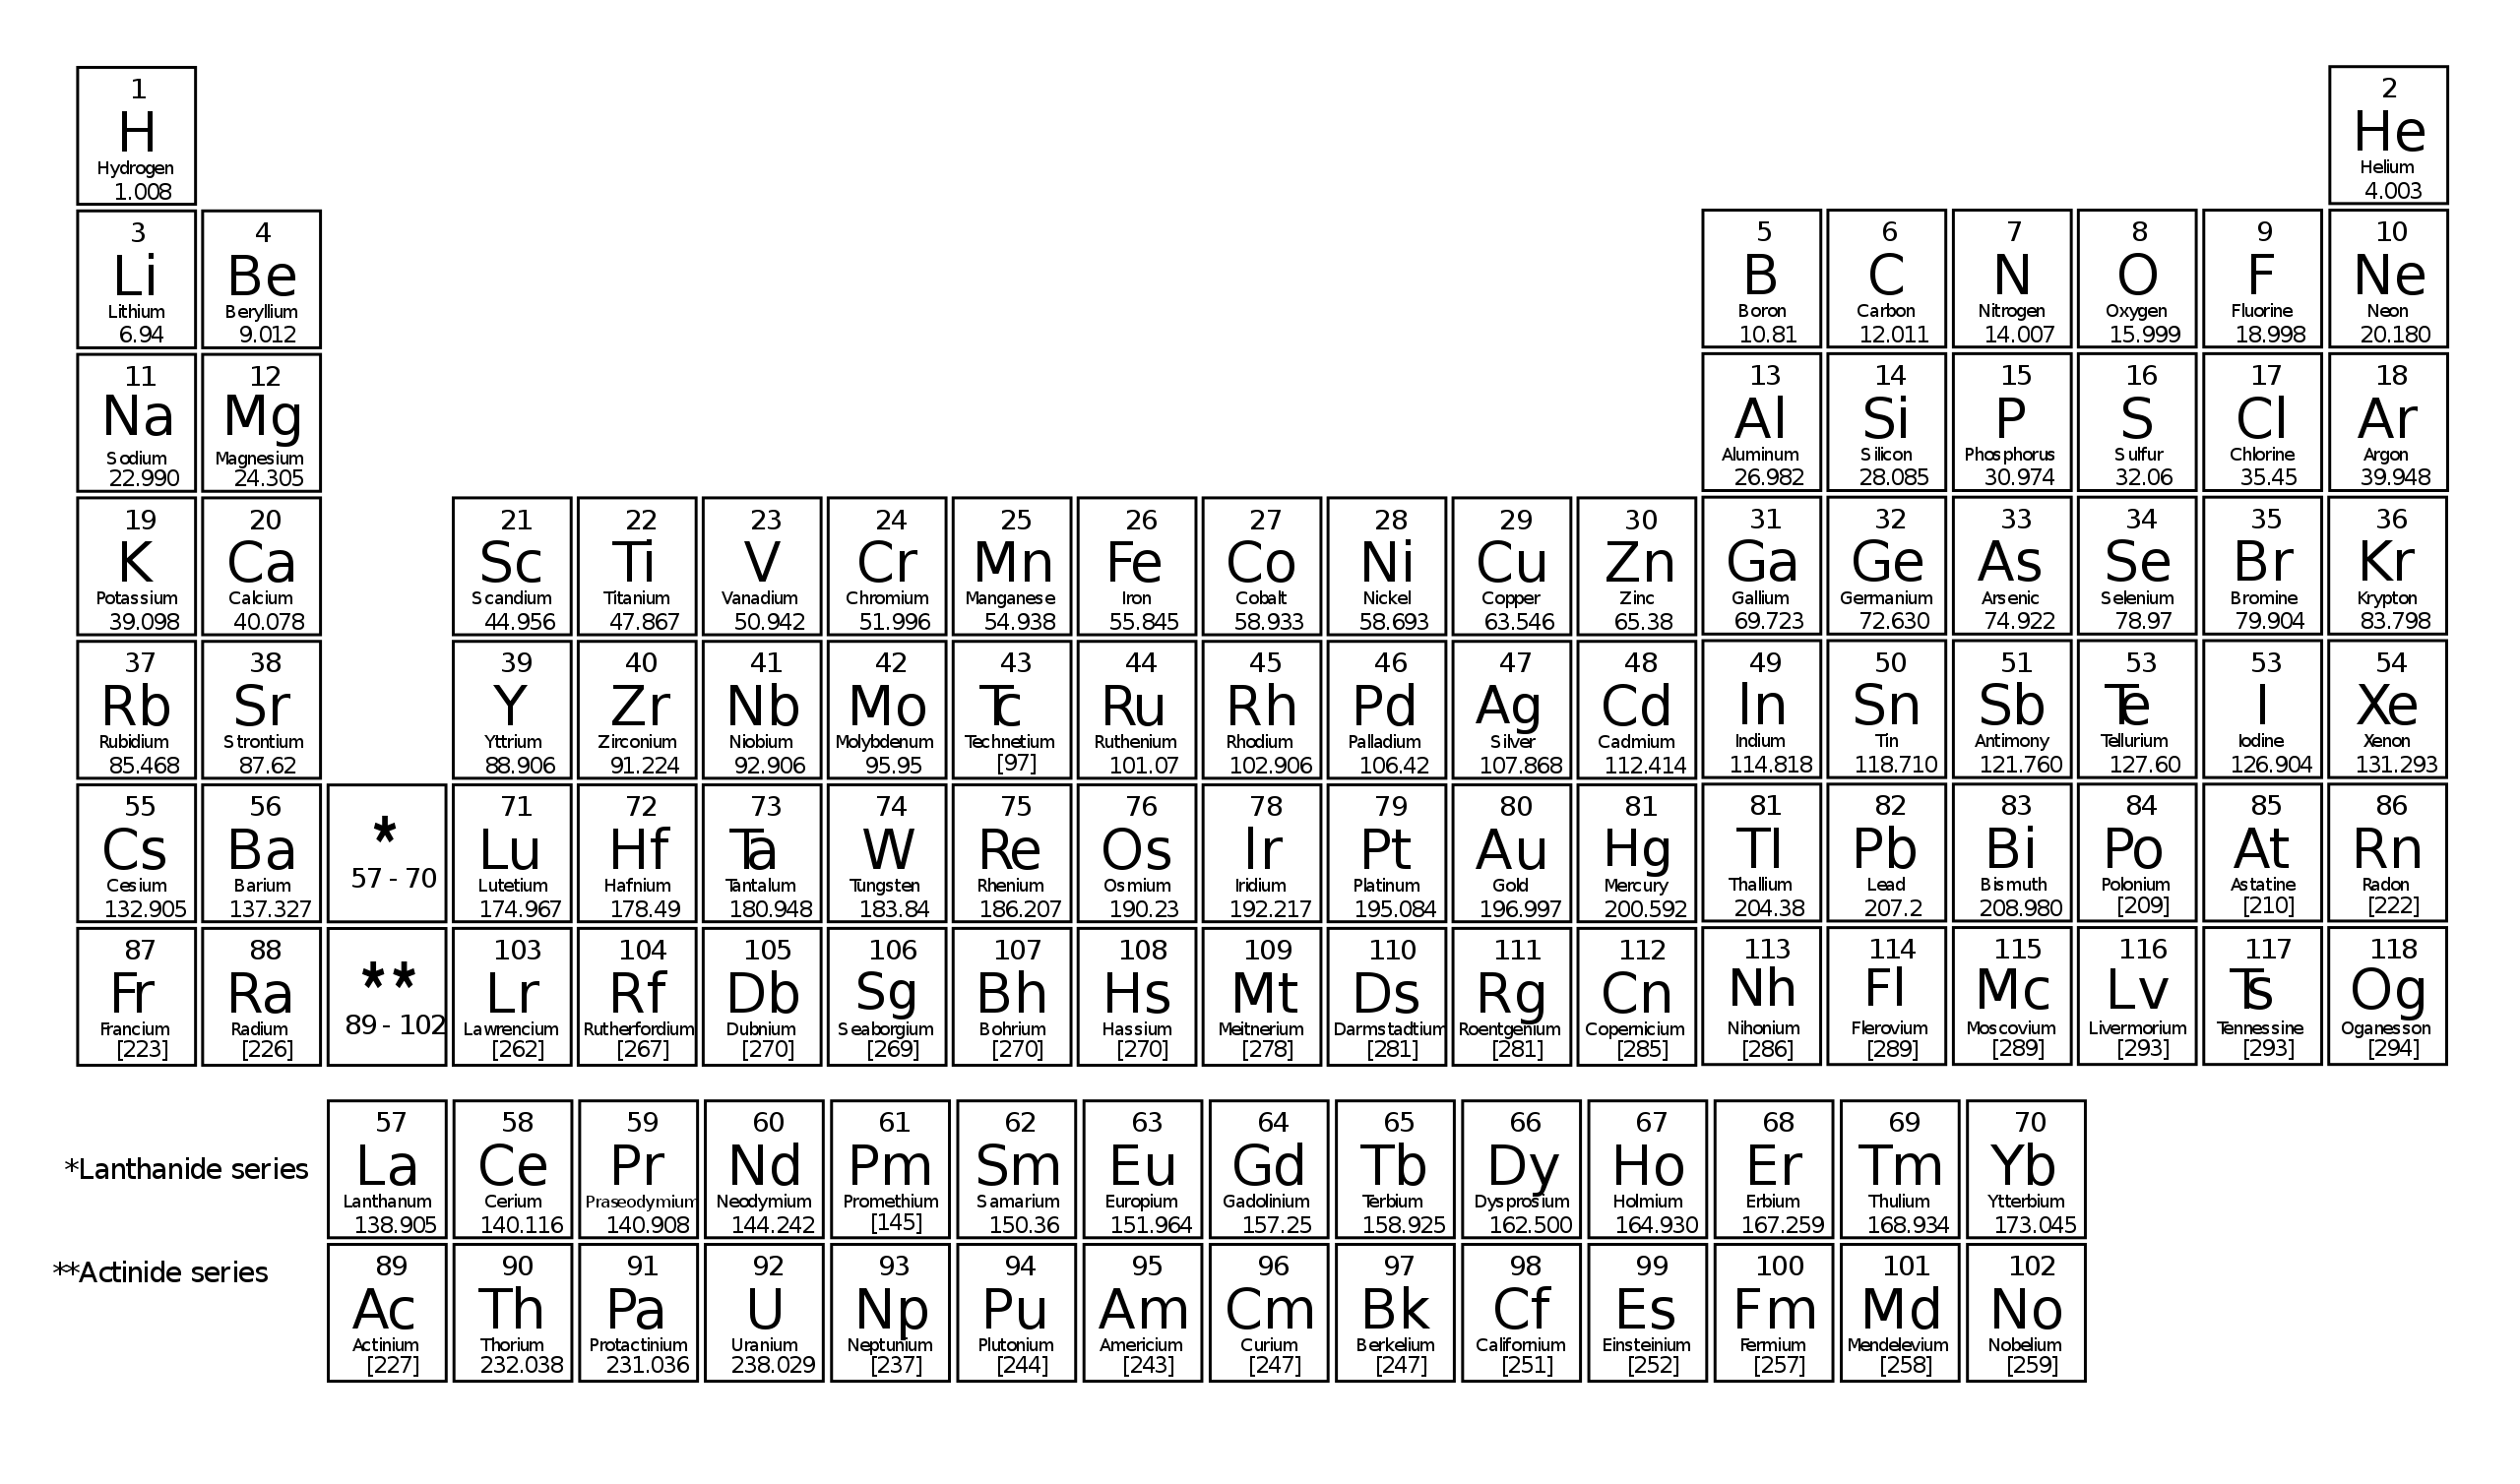
\includegraphics[scale=0.26,angle=90]{periodic_table}
\end{center}

\end{document}
